As explained in Section~\ref{sec:intro} OpenMP 4.0 provides two environment variables OMP\_PROC\_BIND and OMP\_PLACES to help users define the thread placement for their shared memory OpenMP application which together we refer to as \textit{OpenMP Affinity}.%
\begin{figure}[h!]
  \centering
  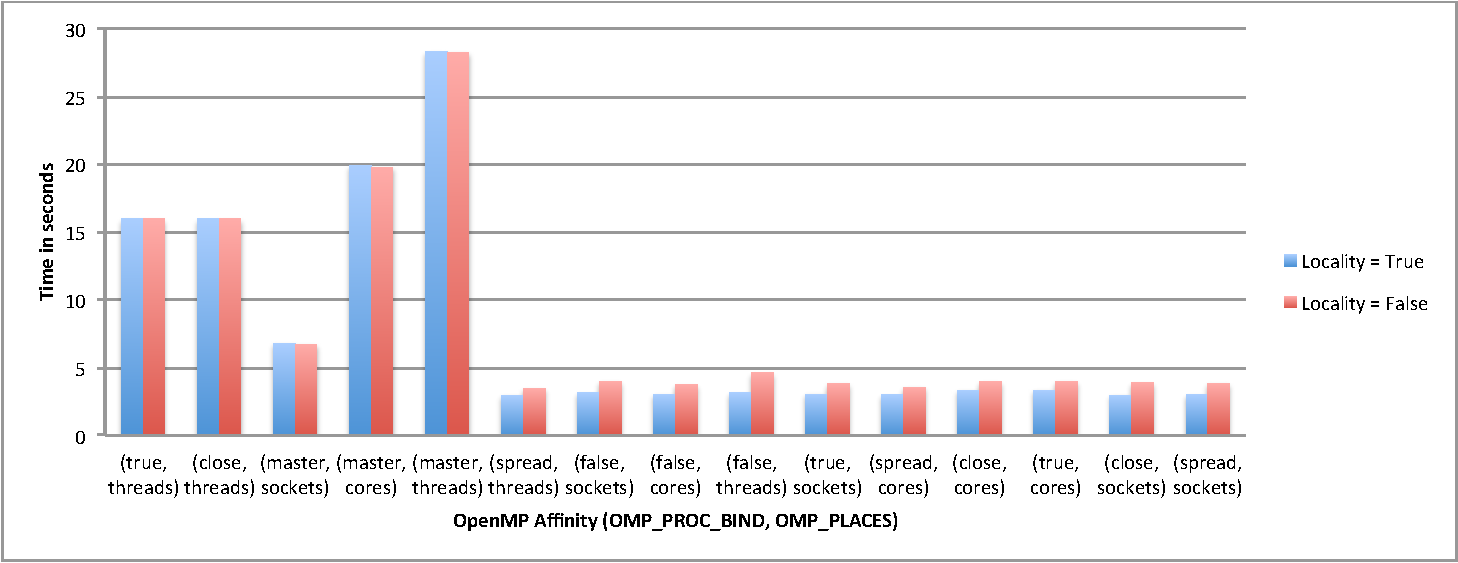
\includegraphics[height=0.4\textwidth, width=0.8\textwidth]{./Images/10Perf.pdf}
       \caption{Performance with 10 OpenMP threads on \textit{Crest}}
       \label{fig:10th}
\end{figure}
%
 We experiment with the locality aware and locality unaware versions of the Jacobi program along with the default first-touch policy to observe the behavior over varying number of threads. 
 For each thread count we record the POWER8 hardware counters and the placement of the threads on the hardware. 
 Figure ~\ref{fig:10th} and ~\ref{fig:20th} shows the performance of 10 and 20 OpenMP threads with different OpenMP Affinity settings respectively. We observed similar results for 40, 80 and 160 OpenMP threads and hence do not show them here.
%
\begin{figure}[h!]
  \centering
  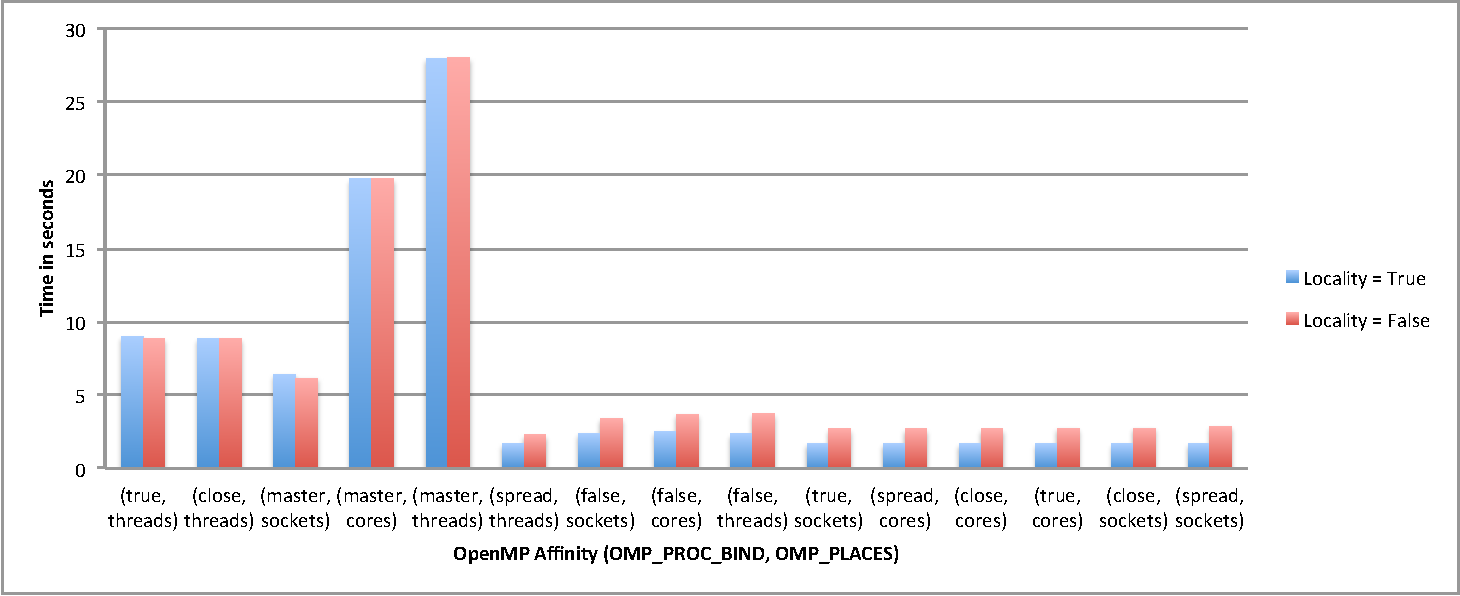
\includegraphics[height=0.4\textwidth, width=0.8\textwidth]{./Images/20Perf.pdf}
       \caption{Performance with 20 OpenMP threads on \textit{Crest}}
       \label{fig:20th}
\end{figure}
%
\begin{figure}[h!]
  \centering
  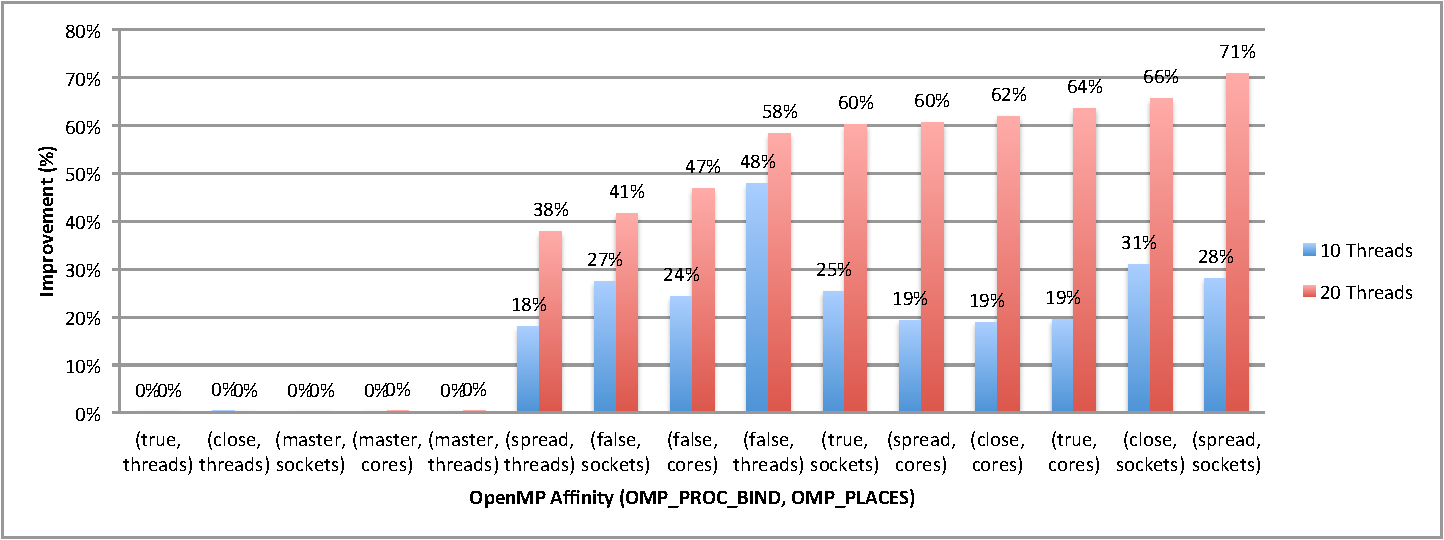
\includegraphics[height=0.4\textwidth, width=0.8\textwidth]{./Images/PerfI.pdf}
       \caption{Comparing Performance Improvement between different number of OpenMP threads}
       \label{fig:imp}
\end{figure}
From the data gathered we observe a similar trend for both 10 and 20 threads. 
For the \textit{(master, threads)} configuration all threads execute on CPUID 0. 
All threads execute in the same core as the master when the configuration is set to \textit{(master, core)}, similarly for \textit{(master, socket)} all threads execute in the same socket. In this case all threads are executing on CPUs 0 through 79 which corresponds to a single NUMA domain. When OMP\_PROC\_BIND set to master we see in Figure ~ref{fig:Imp} that there is no improvement of locality aware algorithms over non-locality aware algorithms (both using the first-touch policy).
For \textit{(close, threads)}, we observe that all OpenMP threads execute on random CPUs between 0-19. All of these cases don't suffer from memory locality issues because they access memory local to the memory within the chip.
In the \textit{(spread, sockets)} and \textit{(close, sockets)} configuration threads are spread across sockets but may be mapped to the same core. We observed that the \textit{(true, threads)} configuration is equivalent to the \textit{(close,threads)} according to the thread mappings.
For all OpenMP affinity settings  with OMP\_PROC\_BIND set to false, threads can migrate and are not bound to a specific thread, core or socket. This migration makes it less impactful on the data placement, but suffers from degraded performance.


%Hardware Counter notes
%We select the cases where we see more improvement for data locality on a given affinity setting 
%Selected cases are (spread, sockets), (spread, cores), master, thread)
%Overall, we see that the two hardware counter that shows the effects of data locality improvements are DMISS_DISTANT, DMISS_L3MISS, 
%We would have expected to see more significnat variation on DMISS_REMOTE, but we found that in some cases, these remote accesses can be cached.
%For the example, the case (spread, sockets) has better DMISS_REMOTE improvement than (spread sockets). In (spread, sockets) some threads (not all) are running
%on the same core, thus sharing local cache lines for (L1, L2) and thus taking advantage of cache reuse for remote data access. This can also be seen by the fact
%of the significant improvement in DMISS_DISTANT which quantifies the stalls by L1 reloads from distant interventions and memory. 
%The improvements we see in (spread, cores) are more on DMISS_L21_L31, which shows a better utilization of the L2/L3 cache as 
%this hardware counter masures the stall cycels by Dcache miss which resolved on chip. In the case of (spread, cores) we are increasing the amount of 
%L2 cache as each thread has access to its own L2 cache on a given core. 
%For the case, of (master, thread), there is very little improvement in the memory subsystem utilization as everything is running on the same thread and the 
%most of the data is local to the socket. In this case the data-locality version doesnt make any difference. This is also true for the case (close, threads) where
% we dont see improvements on the data locality version since data is local to the threads but the threads.


